
% This LaTeX was auto-generated from MATLAB code.
% To make changes, update the MATLAB code and republish this document.

\documentclass{article}
\usepackage{graphicx}
\usepackage{color}

\sloppy
\definecolor{lightgray}{gray}{0.5}
\setlength{\parindent}{0pt}

\begin{document}

    
    

\section*{28. Analytic continuation and convergence acceleration}

\begin{verbatim}
ATAPformats
\end{verbatim}
\begin{par}

We have considered techniques for rational approximation
by best approximation on an
interval (Chapter 24, {\tt remez}),
interpolation or linearized least-squares fitting on an
interval or disk (Chapter 26, {\tt ratinterp} and {\tt ratdisk}),
and Pad\'e approximation at a point or Chebyshev--Pade approximation
on an interval (Chapter 27, {\tt padeapprox} and {\tt chebpade}).
In this final chapter, we turn to the application of such approximations for
extrapolating a function to real or complex values $z$ outside the region
where it is initially known. Three of the applications listed in Chapter
23 fall into this category: those numbered 3 (convergence acceleration for sequences
and series), 4 (determination of poles), and 5 (analytic continuation).

\end{par} \vspace{1em}
\begin{par}
It will be a chapter more of examples than theory. For an example to begin the discussion, suppose we pretend that we can evaluate $$ f(z) = \tanh(z) $$ for real values of $z$ but know nothing about complex values, and we wish to estimate where $f$ has poles.  How might we proceed? (Of course we really know the answer: there are poles at all the odd multiples of $\pm \pi i/2$.)
\end{par} \vspace{1em}
\begin{par}
The first thing to try might be polynomials.  For example, we could use Chebfun to construct a polynomial that approximates $f$ to 16 digits on $[-1,1]$,
\end{par} \vspace{1em}
\begin{par}
 \vskip -2em 
\end{par} \vspace{1em}
\begin{verbatim}
f = @(z) tanh(z); p = chebfun(f); length(p)
\end{verbatim}

        \color{lightgray} \begin{verbatim}ans =
    32
\end{verbatim} \color{black}
    \begin{par}

From here, however, it is hard to make much progress.  As we know from
Chapter~8, $p$ will be a good approximation to $f$ within a certain
Bernstein ellipse, the Chebfun ellipse, which can be plotted by the
command {\tt chebellipseplot}.  We can expect this ellipse to reach
approximately out to the first singularities at $\pm \pi i/2$.  Once we
hit the ellipse, however, everything will change.
According to the theory of Walsh [1959] and Blatt and Saff [1986] mentioned in Chapter~18,
zeros of $p$ will cluster all along the boundary, and a further result of Blatt and
Saff states that outside the ellipse, there will be no convergence at all.  The
polynomial $p$ will simply grow rapidly, its behavior having nothing
to do with that of $f$.  We can confirm this prediction with contour
plots. Here are plots of $|f(z)|$ and $|\kern .7pt p(z)|$ in the upper
half-plane, with black contours at levels $0.25, 0.5, \dots , 3$ and red
contours at $10^1, 10^3, 10^5, \dots, 10^{19}$. We see immediately that
$p$ matches $f$ very well inside the Chebfun ellipse, which is marked in
blue, but not at all outside.

\end{par} \vspace{1em}
\begin{par}
 \vskip -2em 
\end{par} \vspace{1em}
\begin{verbatim}
x = -4:.05:4; y = 0:.05:8;
[xx yy] = meshgrid(x,y); zz = xx + 1i*yy;
ff = f(zz); pp = p(zz);
lev1 = .25:.25:2; lev2 = 10.^(1:2:19);
subplot(1,2,1), hold off, contour(x,y,abs(ff),lev1,'k'), hold on
contour(x,y,abs(ff),lev2,'r'), FS = 'fontsize';
axis([-4 4 0 8]), axis square, title('tanh(z) in upper half-plane',FS,9)
subplot(1,2,2), hold off, contour(x,y,abs(pp),lev1,'k'), hold on
contour(x,y,abs(pp),lev2,'r')
axis([-4 4 0 8]), axis square, title('Degree 29 polynomial approx',FS,9)
chebellipseplot(p,'b','linewidth',2)
\end{verbatim}

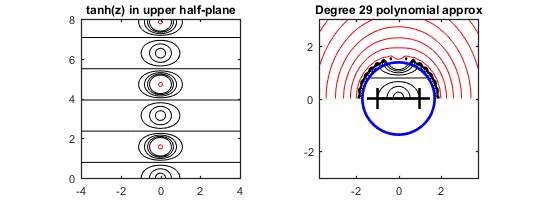
\includegraphics [width=4in]{chap28_01.png}
\begin{par}
 \vskip 1pt 
\end{par} \vspace{1em}
\begin{par}
To get better information, we turn to rational approximation. A practical approach is to use \texttt{ratinterp} to compute rational linearized least-squares approximations of $f$ in $[-1,1]$.  Specifically, suppose we take $r$ to be the type $(7,8)$ approximation to $f$ in 1000 Chebyshev points and draw the same contour plots as before.  The picture changes completely, showing very impressive agreement over most of the range plotted. This is the power and the promise of rational approximation.
\end{par} \vspace{1em}
\begin{verbatim}
d = domain(-1,1);
[p,q,r,mu,nu,poles] = ratinterp(d,f,7,8,1000); rr = r(zz);
subplot(1,2,1), hold off, contour(x,y,abs(ff),lev1,'k'), hold on
contour(x,y,abs(ff),lev2,'r')
axis([-4 4 0 8]), axis square, title('tanh(z) in upper half-plane',FS,9)
subplot(1,2,2), hold off, contour(x,y,abs(rr),lev1,'k'), hold on
contour(x,y,abs(rr),lev2,'r')
axis([-4 4 0 8]), axis square, title('Type (7,8) rational approx',FS,9)
chebellipseplot(p,'b','linewidth',2)
\end{verbatim}

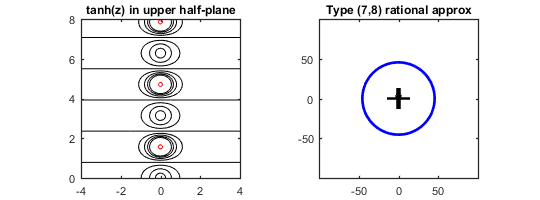
\includegraphics [width=4in]{chap28_02.png}
\begin{par}
 \vskip 1pt 
\end{par} \vspace{1em}
\begin{par}
For a direct measure of the accuracy of $r$ as an approximation to $f$, we can look at $|f(z)-r(z)|$.   In the following plot the contours, from bottom to top, lie at $10^{-14}, 10^{-12}, \dots, 10^{-2}$. Evidently the approximation is excellent over a wide region.
\end{par} \vspace{1em}
\begin{par}
 \vskip -2em 
\end{par} \vspace{1em}
\begin{verbatim}
levels = 10.^(-14:2:-2);
clf, subplot(1,2,1), contour(x,y,abs(ff-rr),levels,'k')
axis([-4 4 0 8]), axis square, title('|tanh(z) - r(z)|',FS,9)
\end{verbatim}

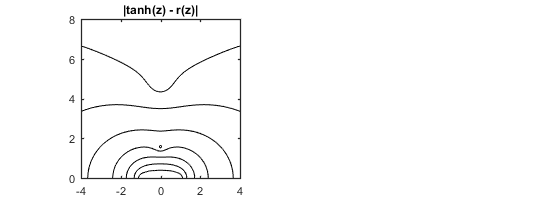
\includegraphics [width=4in]{chap28_03.png}
\begin{par}
 \vskip 1pt 
\end{par} \vspace{1em}
\begin{par}
Results like these become all the more remarkable when one recalls that the problem of analytic continuation is ill-posed: analytic continuations are unique, but they do not depend continuously on the data.  For example, the following observation shows the ill-posedness of the problem of continuing a function analytically from the interval $(-1,1)$ to the unit disk. If $f$ is analytic in the disk, then for any $\varepsilon>0$, there is another function $g$ analytic in the disk such that $\|f-g\|\ge 1$ on the disk and yet $\|f-g\|\le \varepsilon$ on the interval.  (Proof: perturb $f$ by $\varepsilon\sin(Mz)$ for a suitable value of $M$.) Because of this ill-posedness, every successful example of numerical analytic continuation must entail some smoothness assumptions about $f$, whether implicit or explicit. That is to say, numerical analytic continuation always involves some kind of regularization.  (A standard reference on this subject is [Hansen 1998].) In the computations just shown, the regularization is introduced by the use of the SVD in \texttt{ratinterp}.
\end{par} \vspace{1em}
\begin{par}
The question with which we opened the discussion was, where are the poles of $\tanh(z)\kern .7pt$?  To experiment with this, let us now apply \texttt{ratinterp} to compute approximants of types $(2,2), (3,3), \dots , (8,8)$, and examine the poles of these approximations. In the next output, following the convention of the past few chapters, $(m,n)$ represents the permitted type of each approximant and $(\kern .5pt \mu,\nu)$ the exact type, with $\mu\le m$ and $\nu\le n$. Note that $(\kern .5pt \mu,\nu)$ always comes out in the form $(\hbox{odd},\hbox{even})$, because $f$ is an odd function.  Thus there are always an even number of poles, which come in complex conjugate pairs and are pure imaginary, and we print just their positive imaginary parts.
\end{par} \vspace{1em}
\begin{par}
 \vskip -2em 
\end{par} \vspace{1em}
\begin{verbatim}
for n = 2:8
  [p,q,r,mu,nu,poles] = ratinterp(d,f,n,n,1000);
  fprintf('\n(m,n)=(%d,%d), (mu,nu)=(%d,%d):\n',n,n,mu,nu)
  yi = sort(imag(poles)); fprintf('%15.10fi',yi(yi>0))
end
\end{verbatim}

        \color{lightgray} \begin{verbatim}
(m,n)=(2,2), (mu,nu)=(1,2):
   1.8048291471i
(m,n)=(3,3), (mu,nu)=(3,2):
   1.5884736641i
(m,n)=(4,4), (mu,nu)=(3,4):
   1.5716968677i   6.6346803797i
(m,n)=(5,5), (mu,nu)=(5,4):
   1.5708250772i   5.0809800424i
(m,n)=(6,6), (mu,nu)=(5,6):
   1.5707969475i   4.7823013558i  13.7250531659i
(m,n)=(7,7), (mu,nu)=(7,6):
   1.5707963366i   4.7228372782i   9.4126692556i
(m,n)=(8,8), (mu,nu)=(7,8):
   1.5707963295i   4.7161924982i   8.5921524543i  26.1661100394i\end{verbatim} \color{black}
    \begin{par}
The table shows that for larger values of $(m,n)$, two of the poles lie near $1.5707963i$ and $4.71i$. We compare these with the actual first three poles of $\tanh(z)$  in the upper half-plane:
\end{par} \vspace{1em}
\begin{par}
 \vskip -2em 
\end{par} \vspace{1em}
\begin{verbatim}
disp('Exact poles:'), fprintf('%15.10fi',(pi/2)*[1 3 5])
\end{verbatim}

        \color{lightgray} \begin{verbatim}Exact poles:
   1.5707963268i   4.7123889804i   7.8539816340i\end{verbatim} \color{black}
    \begin{par}
Evidently the type $(7,8)$ approximation has captured the first two poles to 9 and 3 digits of accuracy, respectively, numbers that are consistent with the contour levels near $z=1.57i$ and $4.71i$ in the last contour plot.
\end{par} \vspace{1em}
\begin{par}

To understand computations like this, it is important to recognize that
the ``goal'' of $r$ is not to find the poles of $f$, but simply to
approximate $f$ over $[-1,1]$. If $r$ turns out to have poles near those
of $f$, this is a by-product, a side effect that happened because placing
poles there is an effective strategy for approximation.\footnote{Still,
side effects can be the basis of powerful algorithms.  An example is the
Lanczos iteration in numerical linear algebra, which is the standard
method of computing extreme eigenvalues of large symmetric matrices
[Trefethen \& Bau 1997]. Using this method, it is often possible
to find a few dozen eigenvalues of a matrix even if the dimension is in
the millions. Yet at bottom, the Lanczos iteration does nothing but
construct a polynomial to minimize a certain norm.  The accurate
eigenvalues are a by-product of the minimization, since the optimal
polynomial has roots close to some of the eigenvalues of the matrix
[Trefethen \& Greenbaum 1994, Kuijlaars 2006].}  To illustrate this,
suppose we compare the type $(7,8)$ approximation above to one of type
$(15,8)$. One might expect that with more degrees of freedom, the new
approximation would capture the first pole more accurately.  In fact, the
approximation returned has exact type $(15,2)$, and the  accuracy of the
pole has deteriorated, because the denominator is less important to the
quality of the least-squares approximation:

\end{par} \vspace{1em}
\begin{par}
 \vskip -2em 
\end{par} \vspace{1em}
\begin{verbatim}
[p,q,r,mu,nu,poles] = ratinterp(d,f,15,8,1000);
fprintf('\n(m,n)=(15,8), (mu,nu)=(%d,%d):\n',mu,nu)
yi = sort(imag(poles)); fprintf('%15.10fi',yi(yi>0))
\end{verbatim}

        \color{lightgray} \begin{verbatim}
(m,n)=(15,8), (mu,nu)=(15,2):
   1.5707964085i\end{verbatim} \color{black}
    \begin{par}
If we go further and ask for a type $(35,8)$ approximant, \texttt{ratinterp} returns an approximation with no poles at all.  The numerator now provides so much flexibility for the least-squares problem that the degrees of freedom in the denominator are not needed in 16-digit arithmetic, putting us back in the situation of the Chebfun ellipse of the first plot of this chapter.
\end{par} \vspace{1em}
\begin{par}
 \vskip -2em 
\end{par} \vspace{1em}
\begin{verbatim}
[p,q,r,mu,nu,poles] = ratinterp(d,f,35,8,1000);
fprintf('\n(m,n)=(35,8), (mu,nu)=(%d,%d):\n',mu,nu)
\end{verbatim}

        \color{lightgray} \begin{verbatim}
(m,n)=(35,8), (mu,nu)=(25,0):
\end{verbatim} \color{black}
    \begin{par}
One must always bear this in mind when using rational approximations for extrapolation: increasing $m$ and/or $n$ does not always improve the accuracy of the quantities one cares about.
\end{par} \vspace{1em}
\begin{par}
One way to get an idea of the dependence of an approximation on $m$ and $n$ is to print a table of digits of accuracy.  The following table, for example, indicates the number of digits of accuracy in the computed first pole of $\tanh(z)$ for $m = 1,3,5,\dots,19$ and $n = 2,4,6,\dots,20$, all based on robust least-squares fits in 200 Chebyshev points in 16-digit arithmetic.  The table shows again the effect that increasing $m$ beyond a certain small value---moving right in the table---diminishes the accuracy of the pole.
\end{par} \vspace{1em}
\begin{par}
 \vskip -2em 
\end{par} \vspace{1em}
\begin{verbatim}
err = zeros(1,10); disp('DIGITS OF ACCURACY: LEAST-SQUARES')
for n = 2:2:20
  for m = 1:2:19
    [p,q,r,mu,nu,poles] = ratinterp(d,f,m,n,200);
    p1 = imag(poles(abs(poles-1.6i)==min(abs(poles-1.6i))));
    err((m+1)/2) = -round(log10(abs(p1-pi/2)));
  end
  fprintf('%3d',err), disp(' ')
end
\end{verbatim}

        \color{lightgray} \begin{verbatim}DIGITS OF ACCURACY: LEAST-SQUARES
  1  2  3  4  4  5  6  7  7  6 
  1  3  5  6  7  8  8  7  7  6 
  2  4  6  8  9  8  8  7  7  6 
  2  5  8  9  9  8  8  7  7  6 
  3  7  9  9  9  8  8  7  7  6 
  4  8  9  9  9  8  8  7  7  6 
  4  8  9  9  9  8  8  7  7  6 
  5  7  9  9  9  8  8  7  7  6 
  5  7  9  9  9  8  8  7  7  6 
  5  7  9  9  9  8  8  7  7  6 
\end{verbatim} \color{black}
    \begin{par}
The use of rational approximations for locating poles or other singularities has an honorable history.  Many applications are mentioned in the monograph by Baker and Graves-Morris [1996], which is a standard reference on $\hbox{Pad\'e}$ approximation.  One interesting kind of application is to locating singularities of solutions of ODEs or PDEs computed numerically, an idea explored among others by Weideman [2003]. For Chebfun-based explorations, including the application of \texttt{ratinterp} to find complex singularities of solutions to the Lorenz and Lottka--Volterra equations, see $\hbox{[Pach\'on 2010]}$ and [Webb 2012].
\end{par} \vspace{1em}
\begin{par}
Having just mentioned $\hbox{Pad\'e}$ approximation, which was the subject of the last chapter, let us now turn to this alternative method of constructing rational approximations.  Here is a repetition of the last experiment, the table of digits of accuracy in the first pole of $\tanh(z)$, but now based on $\hbox{Pad\'e}$ approximation instead of rational least-squares.  The results are similar, but better. This is not a general conclusion: it depends on the problem.
\end{par} \vspace{1em}
\begin{par}
 \vskip -2em 
\end{par} \vspace{1em}
\begin{verbatim}
disp('    DIGITS OF ACCURACY: PADE')
for n = 2:2:20
  for m = 1:2:19
    [r,a,b,mu,nu,poles] = padeapprox(f,m,n);
    p1 = imag(poles(abs(poles-1.57i)==min(abs(poles-1.57i))));
    err((m+1)/2) = -round(log10(abs(p1-pi/2)));
  end
  fprintf('%3d',err), disp(' ')
end
\end{verbatim}

        \color{lightgray} \begin{verbatim}    DIGITS OF ACCURACY: PADE
  1  2  3  4  5  6  7  8  9 10 
  2  3  5  6  8  9 11 12 13 13 
  2  5  7  9 10 12Inf 11 12 13 
  3  6  8 11 13 14 12Inf 11 12 
  3  7 10 12 14 13 14 12Inf 11 
  4  8 12 14 12 14 13 14 12Inf 
  5  9 13 12 14 12 14 13 14 12 
  5 11 11 13 12 14 12 14 13 14 
  6 12 11 11 13 12 14 12 14 13 
  6 12 12 11 11 13 12 14 12 14 
\end{verbatim} \color{black}
    \begin{par}
In principle, least-squares fitting and $\hbox{Pad\'e}$ approximation are very different techniques, since the first uses function values only at many different points, whereas the second uses values of the function and its derivatives at a single point.  (These are the extreme cases of the general notion of $\hbox{{\em multipoint Pad\'e approximation.})}$ In our actual computation, however, the difference is diminished, because \texttt{padeapprox} begins by computing Taylor coefficients numerically by the FFT based on samples of the function at roots of unity, a standard technique. So in fact, in this comparison, \texttt{ratinterp} and \texttt{padeapprox} both work from function values: the first from samples on $[-1,1]$, the second from samples on the unit circle.  This raises the question, what is achieved by passing through the intermediate stage of Taylor coefficients?  It is a fair point, and indeed, another effective approach would be to solve a rational least-squares problem on the circle directly as in Chapter 26.  Explorations of this kind are presented in $\hbox{[Pach\'on 2010].}$
\end{par} \vspace{1em}
\begin{par}
We now turn to the topic of acceleration of convergence of sequences and series.  The challenge here is as follows. Suppose we know some of the initial terms of a convergent sequence, $$ s_0, s_1, s_2, s_3, \dots \to S, \eqno (28.1) $$ and we want to estimate the limit $S$.  Equivalently, suppose we wish to estimate the limit of an infinite sum, $$ S = a_0 + a_1 + a_2 + \cdots.   \eqno (28.2) $$ The two problems are equivalent since we may regard (28.1) as a sequence of partial sums, $$ s_n = \sum_{k=0}^n a_k, \quad a_k = s_{k+1}-s_k. \eqno (28.3) $$ If the sequence or series converges slowly, how might we speed it up? For example, perhaps we can afford to compute 20 terms, but this gives just 2-digit accuracy. Can we process the data further somehow to improve the accuracy to 6 digits?
\end{par} \vspace{1em}
\begin{par}

There is a long history to such questions, reaching from Stirling and Euler
to the recent tour de force
solution of nine of the ten ``SIAM 100-Digit Challenge'' problems to
10,000 digits of accuracy [Bornemann et al.\ 2004].
It is probably fair to say that almost every method for
accelerating convergence is based on the idea of embedding the sequence
in an analytic function, though this may not be how the original authors
conceived or described their method.

\end{par} \vspace{1em}
\begin{par}

One way in which a sequence might be embedded in an analytic function is
if the terms of the sequence can be regarded as values of a fixed
function at different arguments.  For example, suppose we define a function
$f(z)$ at the points $z = 1, 2^{-1}, 2^{-2}, \dots$ by the formula $f(2^{-k})
= s_k$. Then (28.1) becomes
$$ f(1), f(2^{-1}), f(2^{-2}),  \dots \to S. \eqno (28.4) $$
Does this point of view help us estimate $S$?  The answer will probably
be yes if there exists a function $f$ that is analytic in a neighborhood
of $z=0$ and takes the given values at $z=2^{-k}$.  In such a case, to
estimate $S$, it is enough to interpolate some of the data by a
polynomial $p(z)$ and then compute $p(0)$.  This is the method known as
{\em Richardson extrapolation}, which is of
great practical importance in applications.\footnote{Lewis Fry Richardson
used such ideas as early as 1910, and for a systematic
treatment see his charming article [Richardson 1927].  There are various earlier
roots of Richardson extrapolation too, including Huygens in the 17th century.}
In a typical application,
$h$ might be the mesh size of a numerical discretization and $f(h),
f(h/2), f(h/4),\dots$ the estimates obtained of a quantity of interest as
the mesh is successively refined.  Often only even powers of $h$ appear,
indicating that $f$ is an even function, so one could take the view that
the data are given at $\pm h, \pm h/2, \dots$
and Richardson extrapolation is really
Richardson interpolation.  In the specific case in which
$f(h)$ is an estimate of an integral by the trapezoid or rectangle rule
with step length $h$, this becomes the quadrature method known as {\em
Romberg quadrature}. Nor is the idea of polynomial extrapolation from
data such as (28.4) limited to cases in which the sample points are
related by factors of $2$. If they are $1, 1/2, 1/3,\dots,$ this is
called {\em Salzer extrapolation} [Salzer 1955].

\end{par} \vspace{1em}
\begin{par}
Often, however, the limit of a sequence or series is not in the interior of a region of analyticity of an analytic function. In such a case there may be less mileage in Richardson extrapolation, and one looks for formulations adapted to the edge of a region of analyticity. For such problems, there is a basic starting point: to insert a parameter $z$ in (28.2) so that it becomes the series $$ S(z) = a_0 + a_1z + a_2z^2 + \cdots .  \eqno (28.5) $$ Now we have the problem of evaluating $S(1)$ for a function $S(z)$ with known Taylor coefficients. If (28.2) converges, then $z=1$ is a point of convergence of (28.5), and if (28.2) converges more slowly than geometrically, then $z=1$ must be on the boundary of the disk of convergence of (28.5).  So by introducing a parameter $z$, we have converted the problem of the summation of a slowly convergent series to a problem of evaluating an analytic function at a point on the boundary of the disk of convergence of its Taylor series.
\end{par} \vspace{1em}
\begin{par}
The simplest idea would be to evaluate $S(z)$ for a succession of values of $z$ and use the identity $$ S(1) = \lim_{z\to 1} S(z), $$ where the limit is over real values of $z$ increasing to $1$. This idea is known as \textit{Abel summation} [Hardy 1991].
\end{par} \vspace{1em}
\begin{par}

A more powerful and general approach is to use rational functions,
specifically Pad\'e approximants since the data are given as Taylor
coefficients. Two variants of this idea have received special attention.
We could construct a sequence of type $(m,1)$ Pad\'e approximants, with
one pole, and evaluate them at $z=1$:
$$ r_{01}(1), r_{11}(1), r_{21}(1), \dots. $$
This is called {\em Aitken extrapolation} or {\em Aitken's
$\Delta^2$ method,} used by Aitken [1926] though with
origins further back. Or we could work with type $(n,n)$
Pad\'e approximants,
$$ r_{00}(1), r_{11}(1), r_{22}(1), \dots. $$
This is called {\em epsilon extrapolation} (originally for sequences)
[Shanks 1955, Wynn 1956] or {\em eta extrapolation} (originally for series) [Bauer 1959].
An earlier appearance of essentially the same idea is due
to Schmidt [1941].

\end{par} \vspace{1em}
\begin{par}
Here is an example showing how powerful eta extrapolation can be for some problems.  What is the value of $$ S = \sum_{n=2}^\infty {\sin(n)\over \log(n)} ? $$ The series is extremely slow to converge, as we see by taking partial sums of as many as a million terms:
\end{par} \vspace{1em}
\begin{par}
 \vskip -2em 
\end{par} \vspace{1em}
\begin{verbatim}
S = @(n) sum(sin(2:n)./log(2:n));
disp('    n          S(n)')
for n = 10.^[1:6]
  fprintf('%6.1e   %10.6f\n',n,S(n))
end
\end{verbatim}

        \color{lightgray} \begin{verbatim}    n          S(n)
1.0e+01     0.907319
1.0e+02     0.457822
1.0e+03     0.669234
1.0e+04     0.761940
1.0e+05     0.764913
1.0e+06     0.609190
\end{verbatim} \color{black}
    \begin{par}
To get 10-digit accuracy by summing the series in this fashion, we would need $10^{10000000000}$ terms! The actual answer (not known analytically) is $$ S \approx 0.68391378641828\dots . $$
\end{par} \vspace{1em}
\begin{par}
Here are the diagonal extrapolants, that is, the results of eta extrapolation. Now we just go from $2^1$ to $2^6$ instead of from $10^1$ to $10^6$, yet we get 14 digits of accuracy instead of 1:
\end{par} \vspace{1em}
\begin{par}
 \vskip -2em 
\end{par} \vspace{1em}
\begin{verbatim}
n = 2:150; c = [0 0 sin(n)./log(n)];
disp('  ( n, n)    (mu,nu)          r_nn(1)  ')
disp('  -------    -------        -----------')
for n = 2.^(1:6)
  [r,a,b,mu,nu] = padeapprox(c,n,n,0);
  fprintf('  (%2.0d,%2.0d)    (%2.0d,%2.0d)   %19.15f\n',n,n,mu,nu,r(1))
end
\end{verbatim}

        \color{lightgray} \begin{verbatim}  ( n, n)    (mu,nu)          r_nn(1)  
  -------    -------        -----------
  ( 2, 2)    ( 2, 2)     0.987966950435009
  ( 4, 4)    ( 4, 4)     0.716844624573062
  ( 8, 8)    ( 8, 8)     0.684142517808646
  (16,16)    (16,16)     0.683914704830018
  (32,32)    (32,32)     0.683913786418275
  (64,64)    (64,64)     0.683913786418277
\end{verbatim} \color{black}
    \begin{par}
The convergence is excellent.  Note that we have computed $\hbox{Pad\'e}$ approximants non-robustly by specifying a tolerance of $0$ to \texttt{padeapprox}. In typical applications, this use of non-robust formulas seems advantageous in extrapolation applications, though it brings a risk of sensitivity to noise.  For this example, calling \texttt{padeapprox} with its default tolerance $10^{-14}$ leads to stagnation at type $(15,15)$ with just 7 digits of accuracy.
\end{par} \vspace{1em}
\begin{par}
This simple method of eta extrapolation, at least as implemented by Chebfun's $\hbox{Pad\'e}$ approximation code, can be encapsulated in a single Matlab command we may call \texttt{extrap}.  Given a sequence $a_0, a_1, ..., a_N$, we can round $N/2$ to integers (say, round up for $m$ and down for $n$) and then use \texttt{padeapprox} to compute the type $(m,n)$ $\hbox{Pad\'e}$ approximation $r$.  The accelerated value is then $r(1)$.  Here is the code.
\end{par} \vspace{1em}
\begin{par}
 \vskip -2em 
\end{par} \vspace{1em}
\begin{verbatim}
eval_at_1 = @(r) r(1); N2 = @(c) length(c)/2;
extrap = @(c) eval_at_1(padeapprox(c,ceil(N2(c)),floor(N2(c)),0));
\end{verbatim}
\begin{par}
The $\sin(n)/\log(n)$ example just treated is this:
\end{par} \vspace{1em}
\begin{par}
 \vskip -2em 
\end{par} \vspace{1em}
\begin{verbatim}
extrap([0 0 sin(2:150)./log(2:150)])
\end{verbatim}

        \color{lightgray} \begin{verbatim}ans =
   0.683913786418259
\end{verbatim} \color{black}
    \begin{par}
For another example, suppose we extrapolate the alternating series $$ 1 - {1\over 2} + {1\over 3} - \cdots = \log(2), \eqno (28.6) $$ The result is accurate to machine precision:
\end{par} \vspace{1em}
\begin{par}
 \vskip -2em 
\end{par} \vspace{1em}
\begin{verbatim}
extrap((-1).^(0:30)./(1:31)), exact = log(2)
\end{verbatim}

        \color{lightgray} \begin{verbatim}ans =
   0.693147180559945
exact =
   0.693147180559945
\end{verbatim} \color{black}
    \begin{par}
Note that here, the function $f$ of (28.5) is $\log(1+z)$, so this example shows that eta extrapolation can be effective for functions with branch cuts as well as poles.
\end{par} \vspace{1em}
\begin{par}
Another famous alternating series, which we can obtain by setting $t=0$ in equation (9.3), is $$ 1 - {1\over 3} + {1\over 5} - \cdots = {\pi\over 4}, \eqno (28.7) $$ Again, extrapolation gives machine precision:
\end{par} \vspace{1em}
\begin{par}
 \vskip -2em 
\end{par} \vspace{1em}
\begin{verbatim}
extrap((-1).^(0:30)./(1:2:61)), exact = pi/4
\end{verbatim}

        \color{lightgray} \begin{verbatim}ans =
   0.785398163397448
exact =
   0.785398163397448
\end{verbatim} \color{black}
    \begin{par}
These examples are very impressive, but it is not always so.  For example, here is what happens if we attempt to extrapolate the series $$ \zeta(2) = 1 + {1\over 2^2} + {1\over 3^2} + \cdots = {\pi^2\over 6}, \eqno (28.8) $$
\end{par} \vspace{1em}
\begin{par}
 \vskip -2em 
\end{par} \vspace{1em}
\begin{verbatim}
extrap(1./(1:30).^2), exact = pi^2/6
\end{verbatim}

        \color{lightgray} \begin{verbatim}ans =
   1.639292716362884
exact =
   1.644934066848226
\end{verbatim} \color{black}
    \begin{par}
The convergence is very poor because in this case the function $f(z)$ of (28.5), known as the dilogarithm, has a branch point at $z=1$ itself.  As it happens, this is a case where Salzer extrapolation is effective (Exercise 28.3).
\end{par} \vspace{1em}
\begin{par}
The discussion of convergence acceleration of the last five pages has little in common with the large literature of this subject, because our focus has been solely on the underlying approximations, particularly $\hbox{Pad\'e}$ approximants, and not at all on the mechanics. Our numerical illustrations have utilized the linear algebra of Chapter 27, based on the SVD and requiring $O(n^3)$ floating-point operations to compute a single estimate based on a type $(n,n)$ approximant.  The literature of convergence acceleration is quite different, for it emphasizes recurrence relations and triangular or rhomboidal arrays related to continued fractions that can be used to generate a sequence of approximations at great speed without solving matrix problems.  These approaches are certainly faster, and in fact they may often be more accurate for extrapolation, though they come with a risk of sensitivity to noise and the possibility of breakdown if there is a division by $0$.
\end{par} \vspace{1em}
\begin{par}

A major reason why we have ignored the mechanical or implementational aspects of
convergence acceleration is that these
matters are complicated---and, one might say, distracting.
The differences between various
extrapolation algorithms in practice can be quite intricate, and in a
discussion of such matters, one quickly loses sight of the underlying
mathematics of approximation. For details of these aspects of convergence
acceleration see surveys such as Chapter 3 of
[Baker \& Graves-Morris 1996], [Brezinski \& Redivo Zaglia 1991], [Gragg 1972],
[Joyce 1971], [Sidi 2003], [Weniger 1989], [Wimp 1981], or the appendix
by Laurie in [Bornemann, et al.\ [2004].  Such literature also points
to many further acceleration methods beyond those we have mentioned,
such as Levin's sequence transformation and Brezinski's
theta method.

\end{par} \vspace{1em}
\begin{par}
We finish with an observation that points to exciting further territories of interest to mathematicians at least since Euler. The series (28.5) consists just of Taylor coefficients, so it is meaningful even if the radius of convergence is less than $1$.  Therefore our methods based on analytic continuation can sum divergent series as well as convergent ones. For example, the Taylor series $$ {1\over 1+z} = 1 - z + z^2 - z^3 + \cdots $$ suggests the result $$ 1 - 1 + 1 - 1 + \cdots = {1\over 2} , \eqno (28.9) $$ if we set $z=1$.  Similarly, setting $z = 2$ suggests $$ 1 - 2 + 4 - 8 + \cdots = {1\over 3} . \eqno (28.10) $$ Are these identities actually ``correct''?  As usual in mathematics, the answer depends on what definitions we choose. The formulas (28.9) and (28.10) are not too problematic since they correspond to Taylor series with positive radii of convergence.  In more challenging cases, the series is only asymptotic.  For example, what about this series with factorial coefficients considered by Euler [1760], $$ 0! - 1! + 2! - 3! + \cdots = ~? \eqno (28.11) $$ The factorials grow too fast to be Taylor coefficients for any function analytic in a neighborhood of $z=0$.  However, they are the asymptotic series coefficients at $z=0$ for a function analytic in the right half-plane, namely $$ f(z) = \int_0^\infty {e^{-t}\over 1+zt} \kern .7pt dt. \eqno (28.12) $$ So a plausible candidate for the sum of (28.11) is $$ 0! - 1! + 2! - 3! + \cdots = f(1) = 0.596347362\dots . \eqno (28.13) $$ Our code \texttt{extrap} makes a creditable attempt at computing this number:
\end{par} \vspace{1em}
\begin{par}
 \vskip -2em 
\end{par} \vspace{1em}
\begin{verbatim}
extrap((-1).^(0:10).*factorial(0:10))
\end{verbatim}

        \color{lightgray} \begin{verbatim}ans =
   0.593294558846645
\end{verbatim} \color{black}
    \begin{par}

\begin{displaymath}
\framebox[4.7in][c]{\parbox{4.5in}{\vspace{2pt}\sl
{\sc Summary of Chapter 28.}
Rational approximations provide one of the basic technologies for analytic
continuation and extrapolation.  In particular, Pad\'e approximants are
the basis of standard methods of convergence acceleration for sequences
and series including the Aitken $\Delta^2$, Shanks, epsilon and eta
methods.
\vspace{2pt}}}
\end{displaymath}

\end{par} \vspace{1em}
\begin{par}
\small
\parskip=2pt
\par
{\bf Exercise 28.1.  Contour plot for Taylor polynomials.}
Draw a contour plot like the pair in this chapter for the Taylor polynomial
approximants to $f(z) = \tanh(z)$.  Comment on the result.
\par
{\bf Exercise 28.2.  The divergent factorial series.}
Compute numerically the Pad\'e approximants
$r_{33}, r_{44}, \dots , r_{77}$ for the Taylor coefficients (28.11),
and show that they match $f(1)$ to better than $1\%$, where $f$ is defined by (28.12).
What accuracy do these approximants give for $f(1/2)$?
\par
{\bf Exercise 28.3.  Zeta function.}  It was noted in the text that
eta extrapolation is ineffective for the series (28.8).  Study the behavior
of Richardson and Salzer extrapolation instead.
\par
{\bf Exercise 28.4.  Alternating square roots.}  (a) To 8 digits of accuracy,
what do you think is the limit of $1-1/\sqrt2 + 1/\sqrt 3 - \cdots\,$?
(b) To the same accuracy, what number would you propose as a good
choice for the sum of the divergent series $1-\sqrt2 + \sqrt 3 - \cdots\,$?
\par
{\bf Exercise 28.5.  Approximations to \boldmath$e^z$.}  Compute type
$(1,1)$ approximations to $e^z$ on $[-1,1]$ by
(a) Pad\'e approximation,
(b) best approximation,
(c) Chebyshev--Pad\'e approximation,
(d) Carath\'eodory--Fej\'er approximation,
(e) interpolation in 3 Chebyshev points, and
(f) linearized least-squares approximation in a number of Chebyshev points large
enough to be effectively infinite.  In each case list the coefficients,
measure the $L^2$ and $L^\infty$ errors, and plot the error curve.
\par
{\bf Exercise 28.6.  Nonlinear least-squares approximation.}  Find
a way to compute the true type $(1,1)$ nonlinear least-squares approximation to
$e^z$ on $[-1,1]$, and report the same data for this function as
for the approximations of Exercise 28.7.
\par
{\bf Exercise 28.7.  An alternating series.}
The following identity is known:
$$ 1 + {1\over 2} - {1\over 3}
- {1\over 4} + {1\over 5}
+ {1\over 6} - {1\over 7} - \cdots = {\pi\over 4} + {1\over 2} \log 2.
\eqno (28.14) $$
How many digits do you get by taking $10^1, 10^2, \dots, 10^6$ terms of the series?
Can you get more by extrapolation?

\end{par} \vspace{1em}



\end{document}
    
